\documentclass[conference]{IEEEtran}

\usepackage{cite}
\usepackage{listings}
\usepackage{amsmath}
\lstset{showstringspaces=false, basicstyle=\footnotesize, numbers=left, numbersep=1pt }
\usepackage[tableposition=top]{caption}
\ifCLASSINFOpdf
\usepackage[pdftex]{graphicx}
\usepackage[pdftex]{color}
\usepackage{subcaption}
\else
\fi
\usepackage{url}
\usepackage{upquote}
\usepackage{mdframed}

\hyphenation{op-tical net-works semi-conduc-tor}


\begin{document}\title{SpyREST in Action: An Automated RESTful API Documentation Tool}

\author{\IEEEauthorblockN{S M Sohan, Craig Anslow, and Frank Maurer}
\IEEEauthorblockA{Department of Computer Science\\
University of Calgary\\
Calgary, Alberta T2N 1N4\\
Email: \{smsohan, craig.anslow, frank.maurer\}@ucalgary.ca  }
}
\maketitle


\begin{abstract}
RESTful APIs are often manually documented. As a result, the process is both expensive and error-prone to maintain the documentation of RESTful APIs. In this demonstration paper, we present SpyREST as an automated software as a service tool that can be used to document RESTful APIs. SpyREST leverages a HTTP Proxy server to intercept real API calls to automatically collect and generate RESTful API documentation by synthesizing HTTP traffic involved in API calls. SpyREST provides an automated yet customizable example based documentation solutions for RESTful APIs. RESTful API developers can use SpyREST to automatically generate and maintain updated API documentation.

\end{abstract}

\begin{IEEEkeywords}
RESTful API, Web API, Documentation, Automation, Example based documentation
\end{IEEEkeywords}

\IEEEpeerreviewmaketitle

\section{Introduction}
Fielding introduced RESTful APIs as a versatile mechanism for connecting internet based applications \cite{Fielding_rest}. For example, a hotel web site may use the Google Maps API to provide driving directions to the hotel. RESTful API developers need to provide and maintain API documentations when releasing the APIs so that the APIs can be used. This poses a problem since documentation of RESTful APIs require manual effort and are often less reliable \cite{Espinha_web}.

Automated solutions exist for documentation of local APIs within the context of classes, and methods. For example, JavaDoc can auto generate the documentation for Java APIs. For RESTful APIs, instead of classes and objects, the context of APIs are defined by API endpoints, resources, actions, and example API calls in terms of the HTTP headers, request and response payload formats \cite{Danielsen_validation}. The existing tools do not natively support the different context for RESTful APIs and cannot be readily used to document RESTful APIs.

Our key contribution with SpyREST is providing the necessary tool support to address the unique needs for RESTful API documentation. To this regard, in the next section we have discussed the design goals followed by a HTTP proxy server based prototype implementation to demonstrate an automated RESTful API documentation tool. Then, we presented two use cases to show how API developers can use SpyREST to automatically generate and maintain RESTful API documentation. In the discussion and related work section, we have compared SpyREST against other tools and provided an analysis of how the requirements for SpyREST are derived.

\section{SpyREST}

\subsection{Design} % (fold)
\label{sub:how_it_works}

SpyREST is a web-based software as a service tool\footnote{\url{http://SpyREST.com}}. The design goal for SpyREST is to provide an automated, technology agnostic, and example driven documentation solution for RESTful APIs so that SpyREST can be used a reusable tool to document multiple RESTful APIs. To auto-generate documentation for RESTful APIs, SpyREST relies on HTTP traffic information captured while example API calls are made using a HTTP proxy. The high level process can be described as a 3 step process: API developers make example API calls using a HTTP proxy server, the HTTP proxy server captures the HTTP headers, request and response data, the collected data is synthesized and presented on a web application.

The proxy server used in SpyREST is a specialized one for RESTful API documentation. A typical HTTP proxy server can intercept and record the HTTP traffic for example API calls but further processing is required to generate a usable RESTful API documentation out of the raw HTTP data. For example, API reference documentations need to be version aware so that the documentation can clearly refer to the relevant API versions. To provide human readable description to the example API calls, relevant information needs to be captured in addition to the raw HTTP traffic. Post processing is required to generate the structure of request and response payloads by parsing and consolidating raw HTTP data from multiple example API calls since the optional fields may not be obvious when looked at individual example calls.

To generate usable documentation, SpyREST automatically parses the captured HTTP request and response data and presents summary tables showing the structure for HTTP query parameters, headers, request and response data. For each field, SpyREST displays the name of the field, example values and automatically inferred data type information such as integer, date time, boolean, and string. To reduce verbosity from large API responses, SpyREST automatically strips large responses to only show representative samples from repeated values in arrays. SpyREST does not capture and strip off any authorization header used in the example API calls to prevent confidential information from being part of the documentation.

\begin{figure}[tbh]
  \centering
  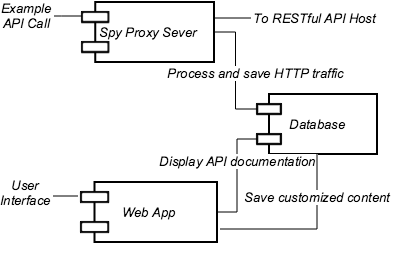
\includegraphics[width=\linewidth]{spyrest_components.png}
  \caption{SpyREST Design}
  \label{fig:components}
\end{figure}

By using a HTTP proxy server, SpyREST enables the documentation of different RESTful APIs independent of the implementation technology behind the APIs. SpyREST can be used both as a software as a service tool or as a self-hosted tool when isolation is desired. SpyREST is released as an open-source product and for self-hosted solutions it can be customized to fit unique requirements.


The web interface of SpyREST provides a hierarchical navigation for RESTful API documentation as follows: each API host has one or more API versions, each API version has one or more resources, each API resource has one or more API actions, each API action may have a structure of HTTP query parameters, headers, request and response payloads as well as many API examples, each API example may have HTTP query parameters, headers, request and response payloads. The web interface also provides a wiki-like editor to allow API developers to override auto generated API documentation using Markdown syntax. On each page, the web interface includes collaboration features so that API developers can discuss questions and collect feedback about specific API documentation pages. For each API example, SpyREST generates a cURL command that can be run to execute the API examples without writing any code.


\subsection{Implementation} % (fold)
\label{sub:implementation}

SpyREST is composed of three main components as shown in Fig. \ref{fig:components}. The ``Spy'' component is the ``value-added'' HTTP proxy server. This component is written using NodeJS. The Spy has internal logic to decode HTTP request URL and headers and auto-detect API versions for the commonly used version identifier patterns. Table \ref{table:versions} shows examples of auto detected versions from accept HTTP header and URL.

\begin{table}[!tbh]
  \caption{Examples of auto detected versions}
  \begin{tabular}{|p{0.2\linewidth}|p{0.5\linewidth}|p{0.2\linewidth}|}
    \hline
    \textbf{Type} & \textbf{Example Value} & \textbf{Detected version}\\
    \hline
    ``accept'' header & application/vnd.ex.ca.v3+json & v3\\
    \hline
    ``accept'' header & application/vnd.ex.ca.v3.1+json & v3.1\\
    \hline
    URL & \url{/v2/x} & v2\\
    \hline
    URL & \url{/v2.1/x} & v2.1\\
    \hline
    URL & \url{/v2.1-pre/users} & v2.1-pre\\
    \hline
  \end{tabular}
  \label{table:versions}
\end{table}

The Spy also parses the URL to auto detect the API resources, API actions and query parameters for the example API calls. For example, given an example API call made to \texttt{GET \url{https://api.github.com/repositories?since=100}}, the Spy automatically detects the API resource as \texttt{repositories}, the API action as \texttt{GET /repositories}, and a query parameter \texttt{since} with an example value of \texttt{100}.

Even though the auto detected API version, resource and actions cover the commonly observed patterns, API developers can override the auto-detections of any of these fields by using custom Spy specific HTTP headers when making the example API calls. The HTTP headers \texttt{x-spy-rest-version}, \texttt{x-spy-rest-resource}, and \texttt{x-spy-rest-action} can be used to override auto-detection of these respective fields. Additionally, API developers can use \texttt{x-spy-rest-desc} header to attach human readable descriptions for each API example so that the web interface can tag the examples against meaningful descriptions.

The Web App component is implemented using Ruby on Rails. To allow RESTful API developers to edit auto generated documentation, the Web App uses the Markdown Syntax. To facilitate collaboration across all the API documentation pages, the Web App uses Disqus, a popular third-party collaboration service, for commenting.

The Spy writes the captured and synthesized API example data into a MongoDB database. The Web App reads and saves custom edits on the same database.

All three SpyREST components are released as Docker containers. Docker is a lightweight virtualization solution that can either be hosted in-house or using many of the popular cloud hosting providers. The public instance of SpyREST has been tested with the three components in three separate docker containers running on a single linux server with 512MB memory, 1 core processor, and 20GB disk space.

\begin{figure*}[!tbh]
  \begin{mdframed}
    \centering
    \begin{subfigure}[t]{0.4\textwidth}
      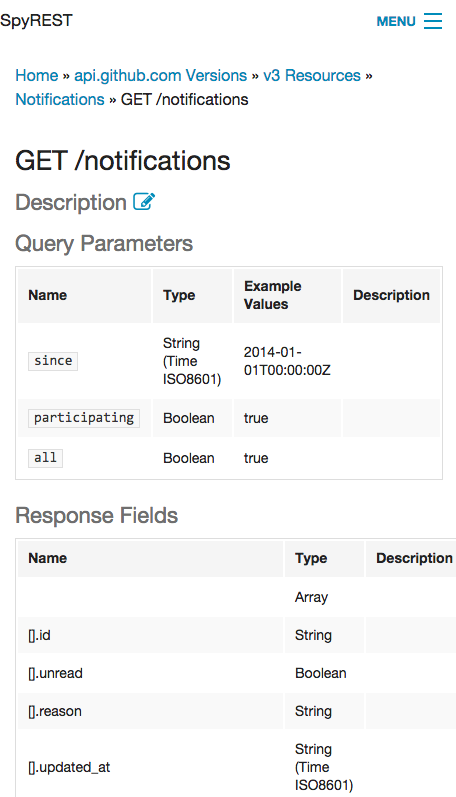
\includegraphics[width=\linewidth]{summary.png}
      \caption{API documentation summary section}
      \label{fig:summary}
    \end{subfigure}
    \begin{subfigure}[t]{0.5\textwidth}
      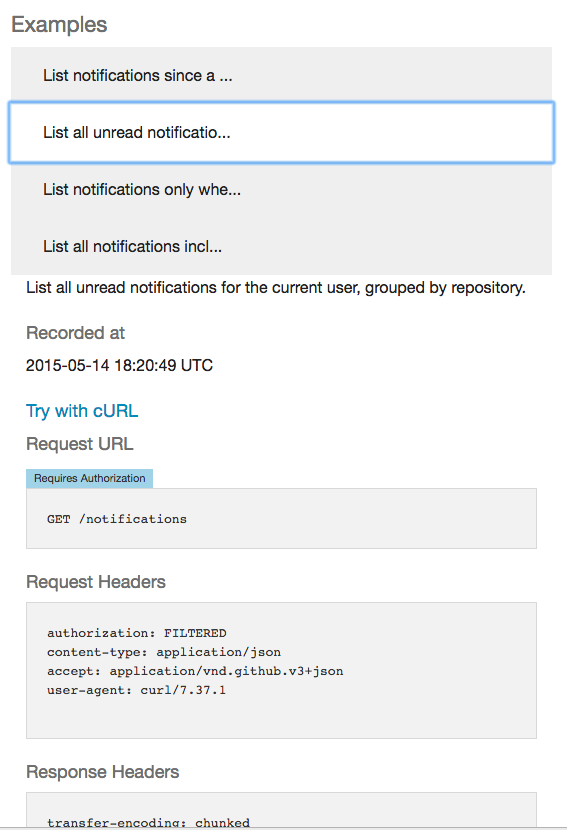
\includegraphics[width=\linewidth]{examples.png}
      \caption{API documentation examples section}
      \label{fig:examples}
    \end{subfigure}
    \caption{SpyREST Screen shots showing auto generated API documentation}
    \label{fig:spyrest_screenshots}
  \end{mdframed}
\end{figure*}

\section{Use Cases}
In this section, we describe two different use cases from the perspective of initially generating a RESTful API documentation for the first time and maintaining the documentation over time as the API evolves.

\subsection{Initial API Documentation} % (fold)
When releasing a RESTful API, API developers need to publish the API documentation so that other developers can use the APIs. For demonstration, consider generating documentation for the ``GET /notifications (List your notifications)'' API that is exposed by GitHub\footnote{\url{https://developer.github.com/v3/activity/notifications/#list-your-notifications}}. Using this API a developer can paginate through the list of all public repositories within GitHub. This API action takes an optional parameter ``since'' that can be used to specify a time filter.

To manually generate documentation for the \texttt{GET /notifications} API, a developer needs to follow these steps: S1) make example authenticated API calls to $GET /notifications$, S2) record the HTTP headers with request and response data, S3) remove duplicate information, S4) remove authentication information, S5) format and stylize the reduced information, S6) add custom content, S7) organize multiple formatted documents together on a web site with navigation, and S8) publish the documentation website. This steps need to be repeated for each of the API endpoints. Since these steps are manually performed, there is also a room for human errors in the aforementioned steps. SpyREST aims to automate all but steps S1 and S6 of this process.

To use SpyREST for auto-generating the documentation of this API, an API developer only needs to make the example API calls via the Spy proxy server with custom HTTP headers for human readable descriptions for the API examples. Custom edits to the auto generated documentation may be made by using the Markdown editor. Fig \ref{fig:spyrest_screenshots} shows a partial screen shot of SpyREST generated documentation for this API given four example API calls. SpyREST fully automates the steps S2-S5, and S7-S8 as follows: S2) the Spy proxy server records the HTTP traffic, S3) the Spy automatically strips off repeated items from the arrays in response body, S4) the Spy does not save any \texttt{Authorization} header, S5) the Web App renders the documentation for all APIs following a consistent look and feel, S7) the Web App provides breadcrumbs for hierarchical navigation of the API objects, S8) the recorded data is automatically published by the Web App in real-time. The API developers only need to focus on finding good example API calls for S1 and describing the complex rules about APIs that are not otherwise derivable from looking at the request and response data alone for S7. In addition to automating the RESTful API documentation process, SpyREST also displays a cURL command for each recorded API example so that developers can try the API examples without having to write any code. Using in page collaboration developers can discuss API related questions and find past conversation all in one place. In this specific example, we see the official documentation of $GET /notifications$ provided by GitHub was outdated and missing several fields (e.g. $subscription\_url$, $repository.releases\_url$, $repository.labels\_url$, $repository.notifications\_url$ and 28 more) that are automatically documented by SpyREST. API developers can also customize the auto generated summary information using a Markdown based editor on SpyREST.

\subsection{Maintaining API Documentation for evolving APIs} % (fold)
Maintenance of RESTful API documentation is another use case of interest since the documentation for RESTful APIs need to evolve with the APIs to reflect the updated information. The 8 steps mentioned previously need to be repeated every time any of the API objects changes when a manual process is followed. Since APIs continue to evolve throughout their lifetime, manually maintaining their documentation incurs further cost or documentation can quickly become outdated.

SpyREST automatically updates the recorded information for each example API call, so rerunning the API examples automatically updates the auto-generated documentation. To uniquely identify each example API call, the Spy computes a digital signature of example API call based on its API version, resource, URL and custom description. To replay the example API calls, API developers can use automated scripts so that once an API example is scripted, it can be run repeatedly. Moreover, the automated scripts can be written as functional tests where the generation of API documentation becomes a side-benefit of running the tests. Running the automated scripts to exercise the API examples frequently can prevent out of date API documentations as shown on the previous use case.

\begin{lstlisting}[language=ruby, breaklines=true, caption={}, label=list:ex, float,floatplacement=H, caption=Example API call using SpyREST, label={lst:notifications}]
class Github

  include HTTParty

  base_uri 'https://api.github.com'
  headers('Accept' => 'application/vnd.github.v3+json',
    'User-Agent' => 'curl/7.37.1',
    'content-type' => 'application/json',
    'Authorization' => "token GITHUB_API_TOKEN'"
  )

  host, port = 'spyrest.com', 9081
  http_proxy host, port

end

describe 'Notifications' do

  it 'List all notifications for the current user, where they are participating, since a time' do

    response = Github.get '/notifications?all=true&participating=true&since=2014-01-01T00:00:00Z'
    assert_equal 200, response.code
  end

end\end{lstlisting}

Listing \ref{lst:notifications} shows an example script written using the Ruby based test framework Minitest. In this example script, the class \texttt{Github} is setup so that the Spy proxy server is used to make example API calls. \texttt{HTTParty} is a third-party library for making RESTful API calls. Then the required headers are setup for using GitHub API. Finally, we setup the proxy connection to SpyREST server. Then, on line 17-25, we define an example API call as an automated test script to generates a documentation for the \texttt{GET /notifications} API action with three query parameters \texttt{all, participating}, and \texttt{since}. The results of the API call can be used to test against expected results. Using this script SpyREST will generate the documentation for this API and auto-update the documentation by rerunning the script anytime the API changes while still providing test coverage.

\section{Discussion}
With SpyREST we have aimed to provide a solution to RESTful API documentation. Manual approach is both expensive and error-prone. SpyREST offers several benefits over existing API documentation tools. We performed a preliminary evaluation of SpyREST by generating documentation of 25 RESTful API actions from 3 different APIs providers (Github.com, KISSMetrics.com, LiquidPlanner.com) using 272 lines of test code\footnote{\url{https://github.com/smsohan/spyrest_examples}}. Comparing SpyREST generated documents against the official documentation (manually generated) we found that the official documentation for 5 of the 25 API actions had outdated response information that didn't match with the actual API responses as captured by SpyREST. This is an expected advantage of automation, since an updated documentation can be produced by replaying existing scripts instead of requiring any manual efforts.

Using automated tests to generate documentation serves a dual purpose for maintaining a test suite since the documentation of the RESTful API becomes an artifact of execution of tests. This is a unique advantage of SpyREST over other API documentation tools that translate manually edited API descriptions into API documents instead of executing actual API calls.

Most general purpose API documentation tools such as JavaDoc extract documentation based on formatted comments from the source code. Since comments are not executable code, manual effort is required to keep the comments updated as the underlying API changes. RESTful API documentation typically includes additional information about HTTP headers, request and response payloads as well as example API calls that are not natively supported by general purpose API documentation tools. Also, general purpose API documentation tools are often programming language specific. SpyREST overcomes these limitations of code comments based API documentation tools by leveraging a HTTP proxy server where executable API examples are converted into API documentation that can be used to document RESTful APIs independent of how the RESTful APIs are implemented.

SpyREST offers unique features compared to other RESTful API documentation services. Swagger\footnote{https://github.com/swagger-api/swagger-spec/blob/master/versions/2.0.md} and Blueprint\footnote{https://github.com/apiaryio/api-blueprint} are two software as a service tools for RESTful API documentation. The key difference between SpyREST and these tools is in the underlying approach used. These tools require the API developers to follow custom vendor specific API specification formats to describe the API objects. Once the APIs are described, the tools can auto-generate the documentations for the APIs. There is no automated tool support to generate the required API description in the vendor specific formats. Thus manual effort is required to produce the required API specifications and maintain it over time. SpyREST does not require on any intermediate API specification since data for documentation is sourced based on live API calls. This eliminates the need for an intermediate step. Unlike SpyREST, Swagger and Blueprint cannot be used as a self-hosted service to document RESTful APIs that cannot be externally shared for confidentiality issues.

The technology choice behind for our implementation of SpyREST components is based on our past experience of using these tools but the concepts behind SpyREST is not dependent on the aforementioned technology choice. As a proof of concept, SpyREST only analyzes JSON based API request and response payloads.

SpyREST is a proof of concept implementation for a novel RESTful API documentation technique. We identify the following limitations. An evaluation with a large number of RESTful APIs as well as evaluation involving API developers is required to understand the strengths and weaknesses of SpyREST. The current implementation of SpyREST only works on JSON based RESTful APIs. SpyREST needs to be enhanced to support other data types such as XML, and CSV. SpyREST, like other HTTP proxy servers, performs an intentional ``man in the middle attack'' to intercept HTTP traffic for example API calls over SSL/TLS. We consider the security impact of this approach to be low since the data is commonly meant to be included in documentation for public use. Otherwise, API developers can use the self-hosted mode and provide SpyREST with the required SSL keys.


\section{Related Work}
Several papers have studied API documentation to understand and recommend requirements for effective API documentation tools. Robillard recommended the following requirements for API documentation: include good examples, be complete, support many complex usage scenarios, be conveniently organized, and include relevant design elements \cite{Robillard_what_makes, Robillard_a_field_study}. Kuhn et al. discussed the importance of examples in API documentation as a key recommendation based on a survey of software developers using APIs \cite{Kuhn_on_designing}. They identified trustworthiness, confidentiality, and limiting information overload as other key recommendations for API documentation. Hoffman et al. recommended providing executable test cases with API documentation \cite{Hoffman_api_documentation}. Nasehi et al. recommended the use of wiki-like editing features for online API documentation to foster collaboration \cite{Nasehi_what_makes}. Parnin et al. and Chen et al. also recommended incorporating collaborative features with API documentations \cite{Parnin_measuring, Chen_who_asked}. Stepalina identified several benefits of using software as a service model for API documentations as follows: cost effective yet powerful, platform agnostic and high accessibility, improved document quality, content re-use, automated tools, and organization of robust and scalable documentation process \cite{Stepalina_saas}.

Several papers have discussed the topic of RESTful API documentation. Espinha et al. found most RESTful API documentations to be less reliable because they are manually generated \cite{Espinha_web}. Danielsen et al. proposed a vocabulary called Web Interface Language (WIfL) for documenting RESTful APIs so that different APIs can be described using a standard terminology \cite{Danielsen_validation}. RESTdesc, RDDL and hRESTS have been proposed as custom specifications to describe RESTful APIs \cite{Verborgh_functional, Mangler_rddl, Kopecky_hrests}. For RESTful API documentation, Myers et al. recommended providing a consistent look-and-feel and an overall map comprising of both text and diagrams, providing a browsing experience with breadcrumb trail following a hierarchy, an effective search interface, providing example code and a way to exercise the examples without writing code.

Our work on SpyREST is a result of following the recommendations as found on the aforementioned related work as well as critically analyzing existing API documentation tools such as JavaDoc, Swagger, and Blueprint, to identify the unmet requirements. Based on our analysis, we incorporated the following recommendations as requirements for SpyREST: automated RESTful API documentation, executable examples, consistent navigation and look and feel, software as a service model, wiki-like editing, automatic stripping of confidential and reducing information overload, and in place collaboration.

\section{Conclusion}
In this paper we have presented SpyREST as a prototype tool to demonstrate an automated solution to RESTful API documentation. Our main contribution is a novel tool that leverages a HTTP proxy server to intercept and automatically extract API documentation from example API calls. SpyREST provides an integrated tool for RESTful API documentation by providing features for automated generation, customization, maintenance, collaboration and executable examples under a single cloud based software as a service platform. By automating the repeated parts of the RESTful API documentation process, SpyREST provides a better alternative to the manual process. API developers can use SpyREST to save the time and cost associated with RESTful API documentation. In future we plan to conduct a quantitative evaluation by using SpyREST to auto generate documentation for a large set of RESTful APIs as well as involving API developers to collect qualitative feedback about the strengths and weaknesses of SpyREST.

\bibliographystyle{IEEEtran}
\bibliography{IEEEabrv,references}


\end{document}


